\documentclass{standalone}
\usepackage{tikz}
\usepackage{xcolor}
\usetikzlibrary{shapes.geometric, arrows, positioning, fit, backgrounds, arrows.meta, calc}

\tikzstyle{csblock} = [rectangle, rounded corners, 
minimum width=3cm, 
minimum height=1cm,
text centered, 
draw=black, 
fill=gray!30]

\tikzstyle{bus-block} = [rectangle, rounded corners, 
minimum width=50cm, 
minimum height=1cm,
text centered, 
draw=black, 
fill=gray!30]


\tikzstyle{extblock} = [rectangle, rounded corners, 
minimum width=3cm, 
minimum height=1cm,
text centered, 
draw=black, 
fill=blue!10]

\tikzstyle{instrument} = [circle, 
minimum width=2cm, 
text centered, 
draw=black, 
fill=gray!30]

\begin{document}
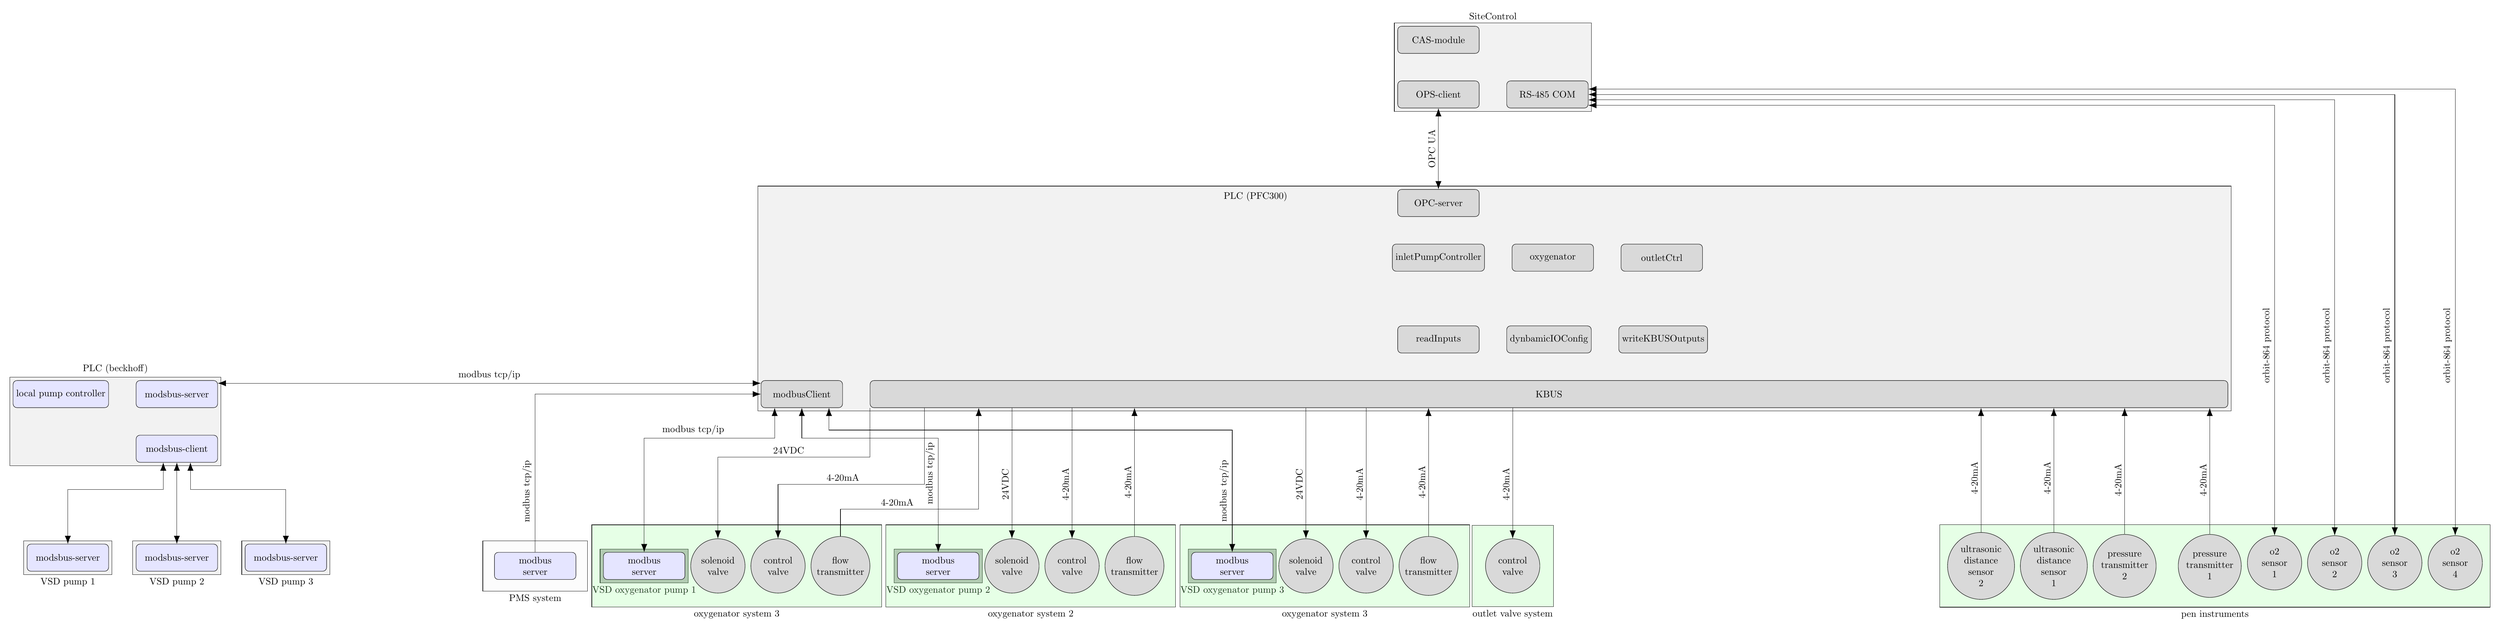
\begin{tikzpicture}[node distance=2cm]

%PLC applications
\node (kbus) [bus-block] {KBUS};
\node (dynkbus) [csblock, above=1cm of kbus ] {dynbamicIOConfig};
\node (readinputs) [csblock,left=1cm of dynkbus ] {readInputs};
\node (pumpctrl) [csblock, above=2cm of readinputs] {inletPumpController};
\node (oxygenator) [csblock, right=1cm of pumpctrl] {oxygenator};
\node (modbus) [csblock, left=1cm of kbus] {modbusClient };
\node (writeoutputs) [csblock, right=1cm of dynkbus] {writeKBUSOutputs};
\node (outletctrl) [csblock, right=1cm of oxygenator] {outletCtrl};
\node (opcServer) [csblock, above=1cm of pumpctrl] {OPC-server};
Add grey background box
\begin{scope}[on background layer]
    \node[fill=gray!10,draw,fit=(kbus)(modbus) (opcServer) (outletctrl) (writeoutputs),label={[xshift=-8.8cm, yshift=-0.7cm]PLC (PFC300)}] {};
\end{scope}

%SCADA
\node (site-cas) [csblock, above = 5cm of opcServer] {CAS-module};
\node (opc-client) [csblock, below=1cm of site-cas] {OPS-client};
\node (rs485) [csblock, right=1cm of opc-client] {RS-485 COM};

%Add grey background box
\begin{scope}[on background layer]
    \node[fill=gray!10,draw,fit=(site-cas) (opc-client) (rs485) ,label=above:SiteControl] {};
\end{scope}

%Pump controller
\node (modbus-server) [extblock, left=20cm of modbus] {modsbus-server};
\node (pump-ctrl) [extblock, left=1cm of modbus-server] {local pump controller};
\node (modbus-client) [extblock, below=1cm of modbus-server] {modsbus-client};
%Add grey background box
\begin{scope}[on background layer]
    \node[fill=gray!10,draw,fit=(modbus-server) (pump-ctrl) (modbus-client) ,label=above:PLC (beckhoff)] {};
\end{scope}

%VSD1
\node (VSD-modbus1) [extblock, below=3cm of modbus-client] {modsbus-server};
%Add grey background box
\begin{scope}[on background layer]
    \node[fill=gray!10,draw,fit=(VSD-modbus1),label=below:VSD pump 2] {};
\end{scope}
%VSD2
\node (VSD-modbus2) [extblock, left=1cm of VSD-modbus1] {modsbus-server};
%Add grey background box
\begin{scope}[on background layer]
    \node[fill=gray!10,draw,fit=(VSD-modbus2),label=below:VSD pump 1] {};
\end{scope}
%VSD3
\node (VSD-modbus3) [extblock, right=1cm of VSD-modbus1] {modsbus-server};
%Add grey background box
\begin{scope}[on background layer]
    \node[fill=gray!10,draw,fit=(VSD-modbus3),label=below:VSD pump 3] {};
\end{scope}


\node (pt1) [instrument, below right = 5cm and -1.5cm of kbus, align=center] {pressure \\ transmitter \\1};
\node (pt2) [instrument, left = .8 cm of pt1, align=center] {pressure \\ transmitter \\2};
\node (usd1) [instrument, left = .2cm of pt2, align=center] {ultrasonic\\distance\\sensor\\1};
\node (usd2) [instrument, left = .2cm of usd1, align=center] {ultrasonic\\distance\\sensor\\2};
\node (out_cv) [instrument, left = 15cm of usd2, align=center] {control\\valve};
\node (o2_1) [instrument, below right = 5cm and 1cm of kbus, align=center] {o2\\sensor\\1};
\node (o2_2) [instrument, right = .2cm of o2_1, align=center] {o2\\sensor\\2};
\node (o2_3) [instrument, right = .2cm of o2_2, align=center] {o2\\sensor\\3};
\node (o2_4) [instrument, right = .21cm of o2_3, align=center] {o2\\sensor\\4};
\node (ft1) [instrument,left=1cm of out_cv, align=center] {flow \\transmitter};
\node (o2_1_cv) [instrument,left=.2cm of ft1, align=center] {control\\valve};
\node (o2_1_s) [instrument,left=.2cm of o2_1_cv, align=center] {solenoid\\valve};
\node (cv_modbus1) [extblock, left=.2cm of o2_1_s, align=center] {modbus\\server};
\node (ft2) [instrument,left=1cm of cv_modbus1, align=center] {flow \\transmitter};
\node (o2_2_cv) [instrument,left=.2cm of ft2, align=center] {control\\valve};
\node (o2_2_s) [instrument,left=.2cm of o2_2_cv, align=center] {solenoid\\valve};
\node (cv_modbus2) [extblock, left=.2cm of o2_2_s, align=center] {modbus\\server};
\node (ft3) [instrument,left=1cm of cv_modbus2, align=center] {flow \\transmitter};
\node (o2_3_cv) [instrument,left=.2cm of ft3, align=center] {control\\valve};
\node (o2_3_s) [instrument,left=.2cm of o2_3_cv, align=center] {solenoid\\valve};
\node (cv_modbus3) [extblock, left=.2cm of o2_3_s, align=center] {modbus\\server};
\node (dsp_modbus) [extblock, left=1cm of cv_modbus3, align=center] {modbus\\server};



\begin{scope}[on background layer]
    \node (x)[fill=gray!50,draw,fit=(cv_modbus1),label=below:VSD oxygenator pump 3] {};
\end{scope}
\begin{scope}[on background layer]
    \node[fill=gray!50,draw,fit=(cv_modbus2),label=below:VSD oxygenator pump 2] {};
\end{scope}
\begin{scope}[on background layer]
    \node[fill=gray!50,draw,fit=(cv_modbus3),label=below:VSD oxygenator pump 1] {};
\end{scope}

\begin{scope}[on background layer]
    \node[fill=green!50,draw,fill opacity=0.2,inner sep=12pt,fit=(ft1) (o2_1_cv) (o2_1_s) (cv_modbus1),label=below:oxygenator system 3] {};
\end{scope}

\begin{scope}[on background layer]
    \node[fill=green!50,draw,fill opacity=0.2,inner sep=12pt,fit= (ft2) (o2_2_cv) (o2_2_s) (cv_modbus2),label=below:oxygenator system 2] {};
\end{scope}

\begin{scope}[on background layer]
    \node[fill=green!50,draw,fill opacity=0.2,inner sep=12pt,fit= (ft3) (o2_3_cv) (o2_3_s) (cv_modbus3),label=below:oxygenator system 3] {};
\end{scope}

\begin{scope}[on background layer]
    \node[fill=green!50,draw,fill opacity=0.2,inner sep=8pt,
    fit= (pt1) (pt2) (usd1) (usd2) (o2_1) (o2_2) (o2_3) (o2_4),
    label=below:pen instruments] {};
\end{scope}

\begin{scope}[on background layer]
    \node[fill=green!50,draw,fill opacity=0.2,inner sep=14pt,fit= (out_cv),label=below:outlet valve system] {};
\end{scope}

\begin{scope}[on background layer]
    \node[fill=gray!10,draw,fill opacity=0.2,inner sep=12pt,fit=(dsp_modbus),label=below:PMS system] {};
\end{scope}

%%%%%%%%%% DRAW %%%%%%%%%%%%%%

%%Draw between FRAMO and VSD's
\draw [{Latex[length=3mm]}-{Latex[length=3mm]}](modbus-client.south) +(-0.5,0) -- +(-0.5,-1) -| (VSD-modbus2.north);
\draw [{Latex[length=3mm]}-{Latex[length=3mm]}](modbus-client.south) -- (VSD-modbus1.north);
\draw [{Latex[length=3mm]}-{Latex[length=3mm]}](modbus-client.south) +(0.5,0) -- +(0.5,-1) -| (VSD-modbus3.north);

%%Draw between FRAMO and Scale
\draw [{Latex[length=3mm]}-{Latex[length=3mm]}]($(modbus-server.east)+(0,0.4)$) -- node[above,midway] {modbus tcp/ip} ($(modbus.west)+(0,0.4)$) ;
%(usd2.north) -- (usd2.north|-kbus.south)

%%Draw between PLC and instruments

\draw [-{Latex[length=3mm]}](usd2.north) -- +(0,4) node[above,midway,rotate=90] {4-20mA} -- (usd2.north|-kbus.south);
\draw [-{Latex[length=3mm]}](usd1.north) -- +(0,4) node[above,midway,rotate=90] {4-20mA} -- (usd1.north|-kbus.south);
\draw [-{Latex[length=3mm]}](pt2.north) -- +(0,4) node[above,midway,rotate=90] {4-20mA} -- (pt2.north|-kbus.south);
\draw [-{Latex[length=3mm]}](pt1.north) -- +(0,4) node[above,midway,rotate=90] {4-20mA} -- (pt1.north|-kbus.south);
\draw [-{Latex[length=3mm]}](ft1.north) -- +(0,4) node[above,midway,rotate=90] {4-20mA} -- (ft1.north|-kbus.south);
\draw [{Latex[length=3mm]}-](o2_1_cv.north) -- +(0,4) node[above,midway,rotate=90] {4-20mA} -- (o2_1_cv.north|-kbus.south);
\draw [{Latex[length=3mm]}-](o2_1_s.north) -- +(0,4) node[above,midway,rotate=90] {24VDC} -- (o2_1_s.north|-kbus.south);
\draw [{Latex[length=3mm]}-{Latex[length=3mm]}](cv_modbus1.north) --node[above,rotate=90] {modbus tcp/ip} +(0,4.5) -| ($(modbus.south)+(1,0)$);
\draw [-{Latex[length=3mm]}](ft2.north) -- +(0,4) node[above,midway,rotate=90] {4-20mA} -- (ft2.north|-kbus.south);
\draw [{Latex[length=3mm]}-](o2_2_cv.north) -- +(0,4) node[above,midway,rotate=90] {4-20mA} -- (o2_2_cv.north|-kbus.south);
\draw [{Latex[length=3mm]}-](o2_2_s.north) -- +(0,4) node[above,midway,rotate=90] {24VDC} -- (o2_2_s.north|-kbus.south);
\draw [{Latex[length=3mm]}-{Latex[length=3mm]}](cv_modbus2.north) -- node[above=0.8cm,rotate=90] {modbus tcp/ip} +(0,4.2) -| ($(modbus.south)+(0,0)$);
\draw [-{Latex[length=3mm]}](ft3.north) -- +(0,1) -| node[above,xshift=-3cm] {4-20mA} ($(kbus.south)+(-21,0)$);
\draw [{Latex[length=3mm]}-](o2_3_cv.north) -- +(0,2)  -| node[above,xshift=-3cm] {4-20mA} ($(kbus.south)+(-23,0)$);
\draw [{Latex[length=3mm]}-](o2_3_s.north) -- +(0,3) -| node[above,xshift=-3cm] {24VDC} ($(kbus.south)+(-25,0)$);
\draw [{Latex[length=3mm]}-{Latex[length=3mm]}](cv_modbus3.north) -- +(0,4.2) -| node[above,xshift=-3cm] {modbus tcp/ip} ($(modbus.south)+(-1,0)$);
\draw [{Latex[length=3mm]}-](out_cv.north) -- +(0,4) node[above,midway,rotate=90] {4-20mA} -- (out_cv.north|-kbus.south);
\draw [-{Latex[length=3mm]}](dsp_modbus) -- +(0,5) node[above,midway,rotate=90] {modbus tcp/ip} |- (modbus);


%% Draw between PLC and SiteControl
\draw [{Latex[length=3mm]}-{Latex[length=3mm]}](o2_1.north) -- +(0,7) node[above,rotate=90] {orbit-864 protocol} |- ($(rs485.east)+(0,-0.4)$);
\draw [{Latex[length=3mm]}-{Latex[length=3mm]}](o2_2.north) -- +(0,7) node[above,rotate=90] {orbit-864 protocol} |- ($(rs485.east)+(0,-0.2)$);
\draw [{Latex[length=3mm]}-{Latex[length=3mm]}](o2_3.north) -- +(0,7) node[above,rotate=90] {orbit-864 protocol} |- ($(rs485.east)+(0,-0.0)$);
\draw [{Latex[length=3mm]}-{Latex[length=3mm]}](o2_4.north) -- +(0,7) node[above,rotate=90] {orbit-864 protocol} |- ($(rs485.east)+(0,0.2)$);

%%Draw between siteControl and PLC
\draw [{Latex[length=3mm]}-{Latex[length=3mm]}](opcServer)  -- node[above,midway,rotate=90]{OPC UA} (opc-client);



\end{tikzpicture}

\end{document}